\subsection{Introduction}

\begin{frame}{Introduction}
\framesubtitle{Internet of Things}
\begin{center}
\makebox[\linewidth]{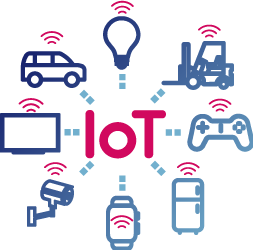
\includegraphics[page=1,width=0.4\paperwidth]{presentation.tex/fig/iot.png}}
\end{center}
\end{frame}

\subsection{LPWAN}

\begin{frame}{Introduction}
\framesubtitle{LPWAN}
\begin{center}
\scalebox{0.6}{%
\begin{tikzpicture}
  \draw[->,thick] (-0.1,0)--(12,0) node[right]{Range};
  \draw[->,thick] (0,-0.1)--(0,8) node[above]{Data Rate};
  \node[] at (1, -0.5) {10m};
  \draw[] (1,-0.1)--(1,0.1);
  \node[] at (3, -0.5) {100m};
  \draw[] (3,-0.1)--(3,0.1);
  \node[] at (5, -0.5) {1km};
  \draw[] (5,-0.1)--(5,0.1);
  \node[] at (7, -0.5) {10km};
  \draw[] (7,-0.1)--(7,0.1);
  \node[] at (9, -0.5) {100km};
  \draw[] (9,-0.1)--(9,0.1);

  \node[] at (-1.2, 1) {1 kbit/sec};
  \draw[] (-0.1,1)--(0.1,1);
  \node[] at (-1.2, 3) {1 Mbit/sec};
  \draw[] (-0.1,3)--(0.1,3);
  \node[] at (-1.2, 5) {100 Mbit/sec};
  \draw[] (-0.1,5)--(0.1,5);
  \node[] at (-1.2, 7) {1 Gbit/sec};
  \draw[] (-0.1,7)--(0.1,7);

  \node[draw,fill=white] at (8,1.5) (lora) {LoRa};
  \node[draw,fill=white] at (8.7,0.8) (sigfox) {SigFox};
  \node[draw,fill=white] at (7.4,2.2) (nb) {NB-IOT};
  \begin{scope}[on background layer]
    \node[draw,fill=blue!30,fit=(lora) (sigfox) (nb), label=above:{LPWAN}] {};
  \end{scope}

  \node[draw,fill=white] at (2.2,3.5) (bluetooth) {Bluetooth};
  \node[draw,fill=white] at (2.7,2.5) (zigbee) {ZigBee};
  \node[draw,fill=white] at (2.0,1.8) (ble) {BLE};
  \begin{scope}[on background layer]
    \node[draw,fill=blue!10,fit=(bluetooth) (zigbee) (ble), label=above:{Short-range}] {};
  \end{scope}

  \node[draw,fill=white] at (3,5) (wifi) {WiFi};
  \begin{scope}[on background layer]
    \node[draw,fill=blue!50,fit=(wifi)] {};
  \end{scope}

  \node[draw,fill=white] at (6.8,5) (lte) {LTE};
  \node[draw,fill=white] at (5.8,6) (5g) {5G};
  \begin{scope}[on background layer]
    \node[draw,fill=blue!60,fit=(lte) (5g), label=above:{Cellular}] {};
  \end{scope}

  \node[] at (6.9,8.2) (leg5) {\small Low};
  \node[draw,fill=blue!10] at (7.5,8.2) (leg1) {};
  \node[draw,fill=blue!30] at (7.8,8.2) (leg2) {};
  \node[draw,fill=blue!50] at (8.1,8.2) (leg3) {};
  \node[draw,fill=blue!60] at (8.4,8.2) (leg4) {};
  \node[] at (10.7,8.2) (leg5) {\small High Power Consumption};
\end{tikzpicture}
}
\end{center}

\end{frame}

\begin{frame}{Introduction}
\framesubtitle{LPWAN}
\begin{columns}
  \begin{column}{0.5\textwidth}
  \begin{itemize}
    \item Longue portée (7-15km)
    \item Faible débit
    \begin{itemize}
      \item $<$ kb/sec
      \item Dizaine de messages par jours
    \end{itemize}
    \item Basse consommation
    \begin{itemize}
      \item Plusieurs années de batterie
    \end{itemize}
    \item Prix faible
    \begin{itemize}
      \item Module à 2.5€
    \end{itemize}
    \item Topologie en étoile
  \end{itemize}
  \end{column}
  \begin{column}{0.5\textwidth}
  \begin{center}
\scalebox{0.6}{
\begin{tikzpicture}[
  radiation/.style={{decorate,decoration={expanding waves,angle=90,segment length=4pt}}},
  ports/.style={
    line width=0.3pt,
    top color=gray!20,
    bottom color=gray!80
  },
  rack switch/.style={
    minimum width=1.25cm,
    minimum height=0.25cm,
    parallelepiped,fill=white, draw,
    parallelepiped offset x=2mm,
    parallelepiped offset y=1.25mm,
    xscale=-1,
    path picture={
      \draw[top color=gray!5,bottom color=gray!40]
      (path picture bounding box.south west) rectangle
      (path picture bounding box.north east);
      \coordinate (A-west) at ([xshift=-0.2cm]path picture bounding box.west);
      \coordinate (A-center) at ($(path picture bounding box.center)!0!(path
        picture bounding box.south)$);
      \foreach \x in {0.275,0.525,0.775}{
        \draw[ports]([yshift=-0.05cm]$(A-west)!\x!(A-center)$)
          rectangle +(0.1,0.05);
        \draw[ports]([yshift=-0.125cm]$(A-west)!\x!(A-center)$)
          rectangle +(0.1,0.05);
       }
      \coordinate (A-east) at (path picture bounding box.east);
      \foreach \x in {0.085,0.21,0.335,0.455,0.635,0.755,0.875,1}{
        \draw[ports]([yshift=-0.1125cm]$(A-east)!\x!(A-center)$)
          rectangle +(0.05,0.1);
      }
    }
  },
  server/.style={
    fill=white, draw,
    minimum width=0.35cm,
    minimum height=0.75cm,
    parallelepiped,
    parallelepiped offset x=3mm,
    parallelepiped offset y=2mm,
    xscale=-1,
    path picture={
      \draw[top color=gray!5,bottom color=gray!40]
      (path picture bounding box.south west) rectangle
      (path picture bounding box.north east);
      \coordinate (A-center) at ($(path picture bounding box.center)!0!(path
        picture bounding box.south)$);
      \coordinate (A-west) at ([xshift=-0.575cm]path picture bounding box.west);
      \draw[ports]([yshift=0.1cm]$(A-west)!0!(A-center)$)
        rectangle +(0.2,0.065);
      \draw[ports]([yshift=0.01cm]$(A-west)!0.085!(A-center)$)
        rectangle +(0.15,0.05);
      \fill[black]([yshift=-0.35cm]$(A-west)!-0.1!(A-center)$)
        rectangle +(0.235,0.0175);
      \fill[black]([yshift=-0.385cm]$(A-west)!-0.1!(A-center)$)
        rectangle +(0.235,0.0175);
      \fill[black]([yshift=-0.42cm]$(A-west)!-0.1!(A-center)$)
        rectangle +(0.235,0.0175);
    }
  },
  antenna/.pic={
    code={\tikzset{scale=2/10}
      \draw[semithick] (0,0) -- (1,4);% left line
      \draw[semithick] (3,0) -- (2,4);% right line
      \draw[semithick] (0,0) arc (180:0:1.5 and -0.5);
      \node[inner sep=4pt] (circ) at (1.5,5.5) {};
      \draw[semithick] (1.5,5.5) circle(8pt);
      \draw[semithick] (1.5,5.5cm-8pt) -- (1.5,4);
      \draw[semithick] (1.5,4) ellipse (0.5 and 0.166);
      \draw[semithick,radiation,decoration={angle=45}] (1.5cm+8pt,5.5) -- +(0:2);
      \draw[semithick,radiation,decoration={angle=45}] (1.5cm-8pt,5.5) -- +(180:2);
    }
  },
  node/.pic={
    code={\tikzset{scale=2/10}
      \draw[semithick] (1.5,-0.5) -- (1.5,1.5cm-8pt);
      \draw[semithick] (1.5,1.5) circle(8pt);
      \draw[semithick,radiation,decoration={angle=45}] (1.5cm+8pt,1.5) -- +(0:3);
      \draw[semithick,radiation,decoration={angle=45}] (1.5cm-8pt,1.5) -- +(180:3);
    }
  }
]
  \draw[color=blue!20,fill=blue!20] (-1.8,2) circle (2.8cm);
  \draw[color=blue!20,fill=blue!20] (-1.8,0) circle (2.3cm);
  \draw[color=blue!20,fill=blue!20] (-1.8,-2) circle (2.8cm);

  \path (0.5,0) edge [-,semithick,draw=gray!70] (2,0);
  \path (2,0) edge [-,semithick,draw=gray!70] (4,2);
  \path (2,0) edge [-,semithick,draw=gray!70] (4,0);
  \path (2,0) edge [-,semithick,draw=gray!70] (4,-2);

  \path (0,-0.4) pic [fill=white,scale=1] {antenna};

  \path (-2,2) pic [black,scale=0.8] {node};
  \path (-2,0) pic [black,scale=0.8] {node};
  \path (-2,-2) pic [black,scale=0.8] {node};

  \node[rack switch] at (2,0) {};

  \node[server] (loraserv) at (4,0) {};
  \node[server] (loraserv) at (4,2) {};
  \node[server] (loraserv) at (4,-2) {};
\end{tikzpicture}
}
\end{center}
 
    
  \end{column}
\end{columns}
\end{frame}

\subsection{Network Stack}

\begin{frame}{Introduction}
\framesubtitle{Network Stack}
\begin{center}
\scalebox{0.8}{%
\begin{tikzpicture}[auto,node distance=1.2cm]
  \tikzstyle{comment}=[ right=2pt, font=\small, fill=white, text=black, draw=black, ]
  \tikzstyle{every state}=[rectangle,thick,draw=black,fill=gray!20,text=black, minimum width= 6cm, minimum height= 1.00cm ]
  \tikzstyle{smallstate}=[rectangle,thick,draw=black!80,fill=gray!10,text=black, minimum width= 6cm, minimum height= 0.25cm ]
  \tikzstyle{innerstate}=[rectangle,thick,draw=black,fill=gray!10,text=black, minimum width= 4cm, minimum height= 1.00cm ]

  \only<1>{
    \node[state] at (0, 0) (A)                  {Application Layer};
    \node[state]         (B) [below of=A]       {Presentation Layer};
    \node[state]         (C) [below of=B]       {Session Layer};
    \node[state]         (D) [below of=C]       {Transport Layer};
    \node[state]         (E) [below of=D]       {Network Layer};
    \node[state]         (F) [below of=E]       {Data Link Layer (MAC+LLC)};
    \node[state]         (G) [below of=F]       {Physical Layer};
    \draw[decorate,decoration={brace,amplitude=8pt},xshift=-5pt,yshift=0pt,black!50] (D.south west) -- (B.north west) node[black!50,midway,left,xshift=-26pt] {\tiny Abstraction};
  }

  \only<2>{
    \node[state] at (0, 0) (A)                  {Application Layer};
    \node[smallstate]    (B) [below of=A]       {...};
    \node[state]         (E) [below of=B]       {Network Layer};
    \node[state]         (F) [below of=E]       {Data Link Layer (MAC+LLC)};
    \node[state]         (G) [below of=F]       {Physical Layer};
    \draw[decorate,decoration={brace,amplitude=8pt},xshift=-5pt,yshift=0pt,white] (D.south west) -- (B.north west) node[white,midway,left,xshift=-26pt] {\tiny Abstraction};

    \draw[decorate,decoration={brace,amplitude=8pt},xshift=-5pt,yshift=0pt,black!70] (E.south west) -- (E.north west) node[black!70,midway,left,xshift=-6pt] {\tiny Internet Integration};
    \draw[decorate,decoration={brace,amplitude=8pt},xshift=-5pt,yshift=0pt,black!70] (F.south west) -- (F.north west) node[black!70,midway,left,xshift=-6pt] {\tiny Access};
    \draw[decorate,decoration={brace,amplitude=8pt},xshift=-5pt,yshift=0pt,black!70] (G.south west) -- (G.north west) node[black!70,midway,left,xshift=-6pt] {\tiny Radio Comm};
  }

\end{tikzpicture}
}
\end{center}

\end{frame}

\begin{frame}{Introduction}
\framesubtitle{Network Stack}
\begin{center}
\scalebox{0.8}{%
\begin{tikzpicture}[auto,node distance=1.2cm]
  \tikzstyle{comment}=[ right=2pt, font=\small, fill=white, text=black, draw=black, ]
  \tikzstyle{every state}=[rectangle,thick,draw=black,fill=gray!20,text=black, minimum width= 6cm, minimum height= 1.00cm ]
  \tikzstyle{smallstate}=[rectangle,thick,draw=black!80,fill=gray!10,text=black, minimum width= 6cm, minimum height= 0.25cm ]
  \tikzstyle{innerstate}=[rectangle,thick,draw=black,fill=gray!10,text=black, minimum width= 4cm, minimum height= 1.00cm ]

  \node[state] at (0, 0) (A)                  {Application};
  \node[smallstate]    (B) [below of=A]       {...};
  \node[state]         (E) [below of=B]       {Network};
  \node[state]         (F) [below of=E]       {Data Link};
  \node[state]         (G) [below of=F]       {Physical};
  \draw[decorate,decoration={brace,amplitude=8pt},xshift=-5pt,yshift=0pt,white] (D.south west) -- (B.north west) node[white,midway,left,xshift=-26pt] {\tiny Abstraction};

  \draw[decorate,decoration={brace,amplitude=8pt},xshift=-5pt,yshift=0pt,black!70] (E.south west) -- (E.north west) node[black!70,midway,left,xshift=-6pt] {\tiny Internet Integration};
  \draw[decorate,decoration={brace,amplitude=8pt},xshift=-5pt,yshift=0pt,black!70] (F.south west) -- (F.north west) node[black!70,midway,left,xshift=-6pt] {\tiny Access};
  \draw[decorate,decoration={brace,amplitude=8pt},xshift=-5pt,yshift=0pt,black!70] (G.south west) -- (G.north west) node[black!70,midway,left,xshift=-6pt] {\tiny Radio Comm};
\end{tikzpicture}
}
\end{center}

\end{frame}
